\subsection{Comparison with theoretical models} \label{sec:WBoson_Results_ComparisonWithTheory}

The measurements of the \Wb-boson production in \RunpPb collisions at \SI{8.16}{\TeV} are compared to three NLO PDF calculations. In all three PDF calculations, the isospin effect is taking into account for the \Pb nucleus. A description of each PDF model is provided below:

\begin{itemize}

 \item CT14: this model assumes no nuclear modifications and uses the NLO CT14 proton PDF for both the incoming proton and \Pb-ion.

 \item CT14+EPPS16: this PDF model employs the CT14 PDF for the incoming proton and apply the EPPS16 nuclear corrections on the CT14 PDF for the incoming \Pb-ion.

 \item CT14+nCTEQ15: this PDF model makes use of the CT14 PDF for the incoming proton and the nCTEQ15 nuclear PDF for the incoming \Pb-ion.

\end{itemize}

The results of the PDF models are derived using the parton-level Monte Carlo program MCFM~\cite{MCFM}. The comparison between the PDF calculations and the data are shown in \fig{fig:CrossSection_WToMu_PA_Model} for the \WToMuNu differential cross sections, in \fig{fig:ChargeAsymmetry_WToMu_PA_Model} for the muon charge asymmetry and in \fig{fig:ForwardBackwardRatio_WToMu_PA_Model} for the forward-backward ratios. In all figures, the results of the CT14 PDF model calculations are shown using continuous lines, while the CT14+EPPS16 and CT14+nCTEQ15, are shown with green and brown dashed lines, respectively.

As can be seen in \fig{fig:CrossSection_WToMu_PA_Model}, the \WToMuNu cross section measurements at forward rapidity favour the PDF calculations including nuclear modifications, while at backward rapidity all three PDF calculations are in good agreement with the data. Moreover, in the case of the muon charge asymmetry shown in \fig{fig:ChargeAsymmetry_WToMu_PA_Model}, the results of the theory calculations derived using the CT14 proton PDF only, and those including the EPPS16 nuclear modifications, are in good agreement with the measurements, while the nCTEQ15 nPDF calculations expect a slightly larger muon charge asymmetry in the most backward \etaMuCM range. Finally, from the ratios of the signal event yields at forward-over-backward \etaMuCM displayed in \fig{fig:ForwardBackwardRatio_WToMu_PA_Model}, the nuclear PDF calculations describe much better the data compared to the free-nucleon PDF calculation.

\begin{figure}[htb!]
 \centering
 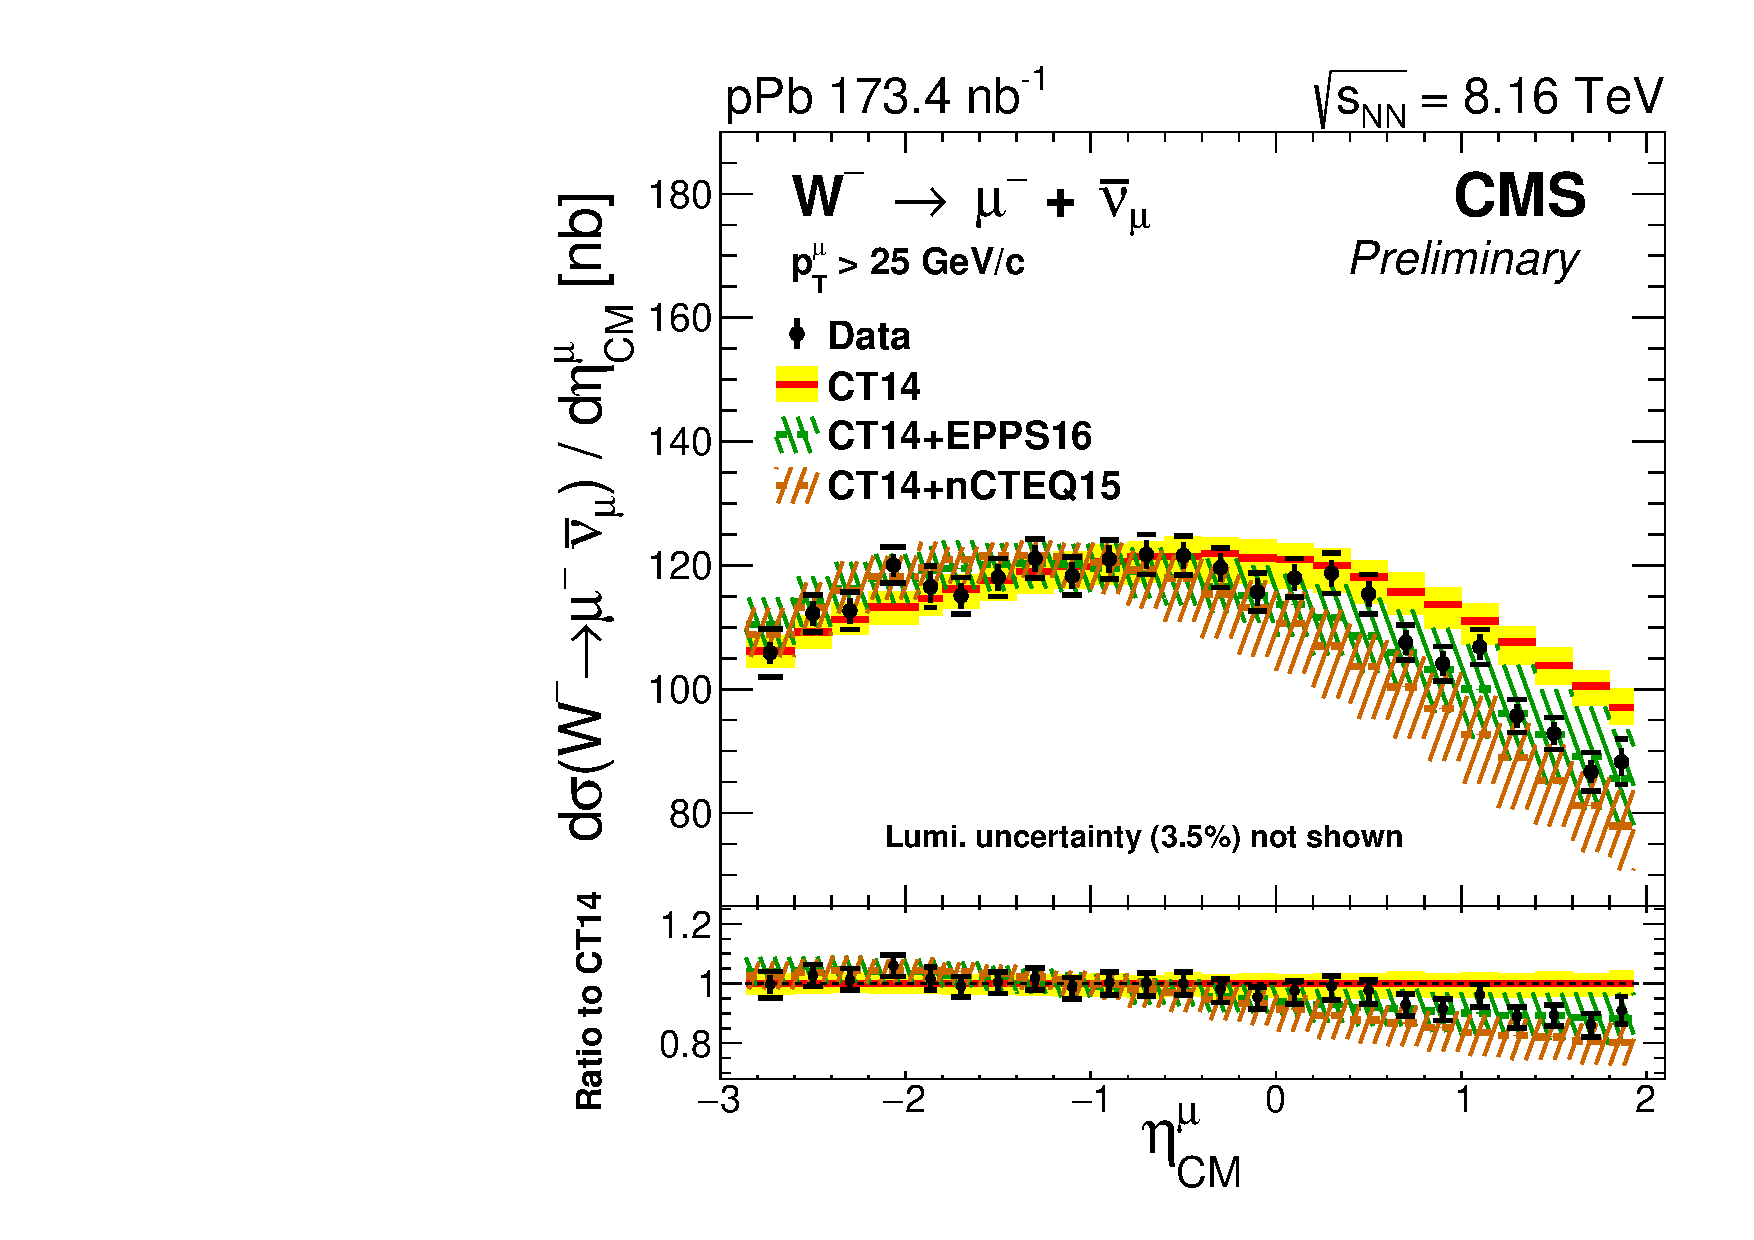
\includegraphics[width=0.45\textwidth]{Figures/WBoson/Results/Theory/gr_WToMuMi_PA_Cross_Section_EffTnP_NominalWithTheoryAndRatio.pdf}
%%
 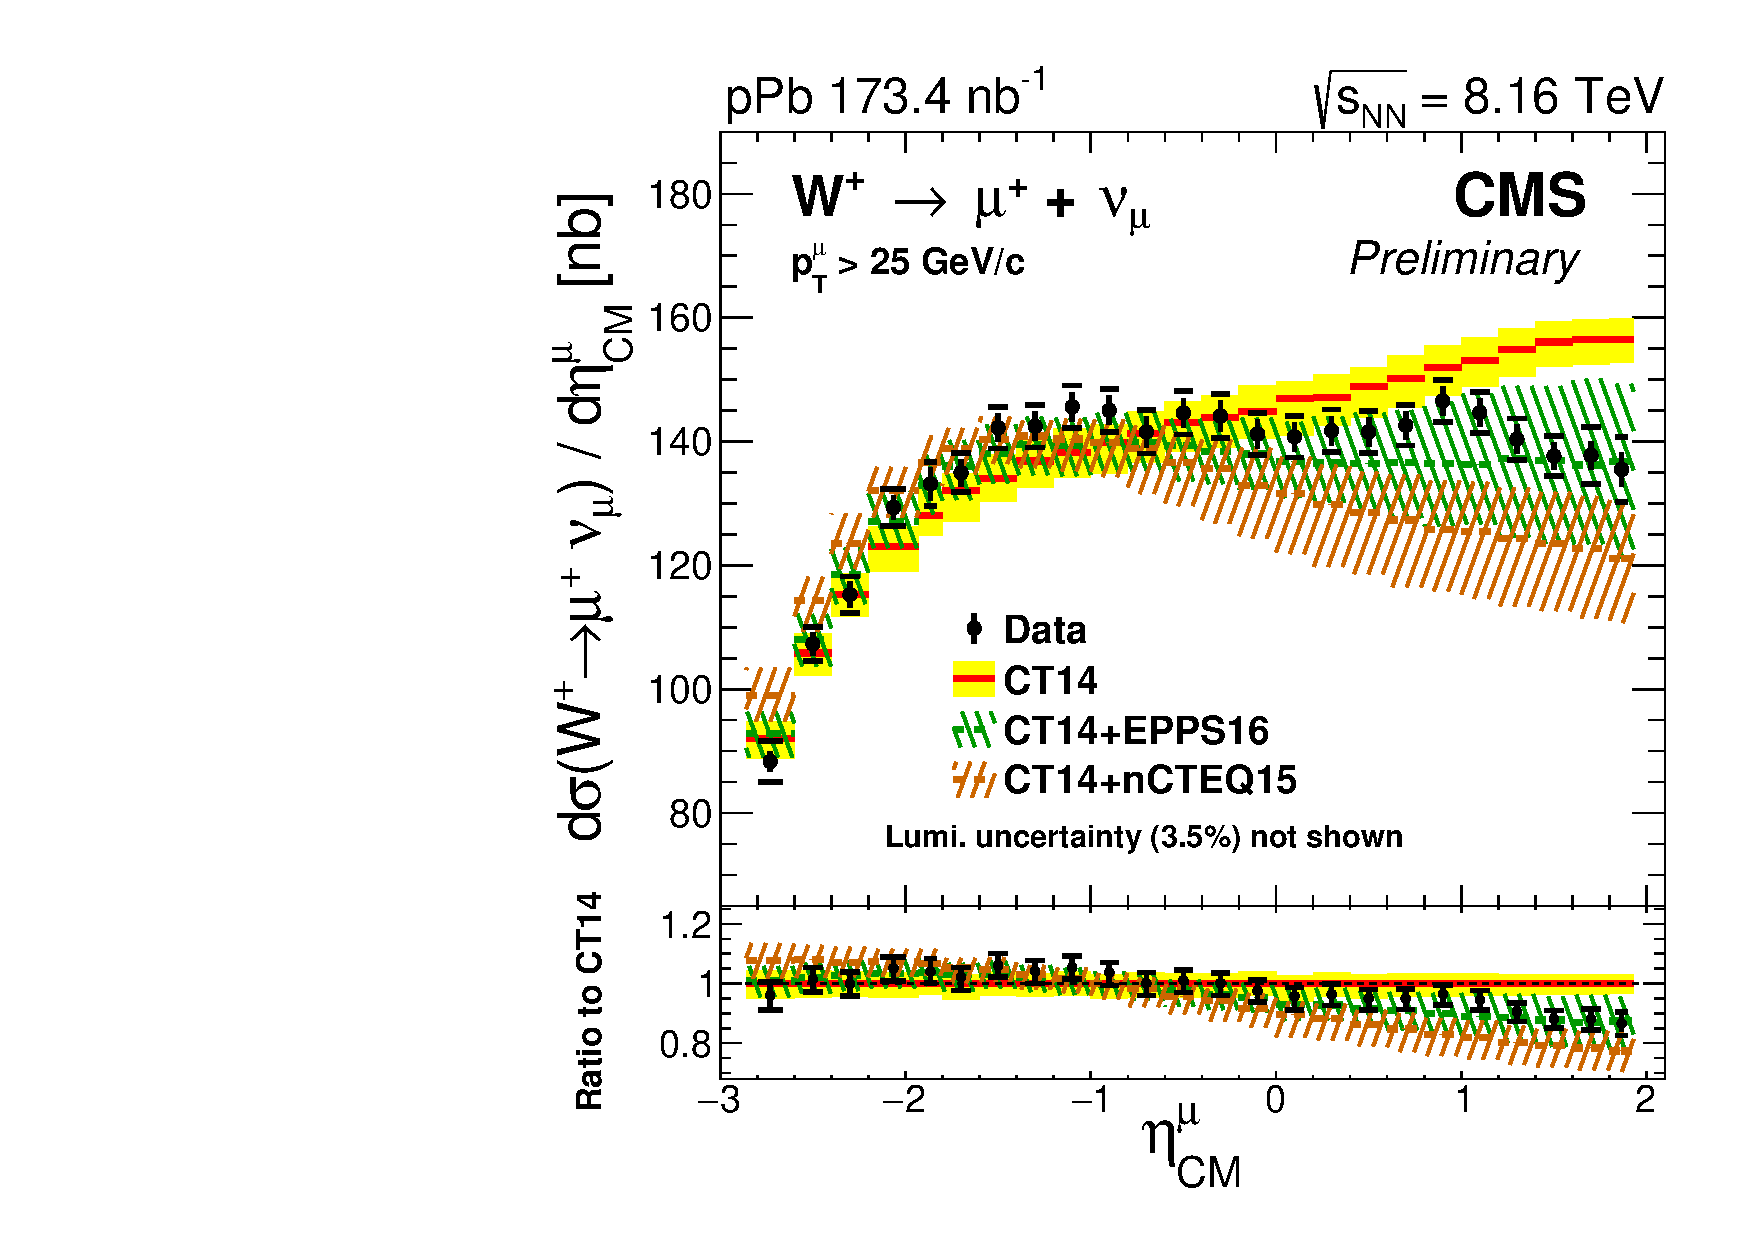
\includegraphics[width=0.45\textwidth]{Figures/WBoson/Results/Theory/gr_WToMuPl_PA_Cross_Section_EffTnP_NominalWithTheoryAndRatio.pdf}
 \caption{Differential cross sections for \WToMuNuPl (left) and \WToMuNuMi (right), as a function of the muon \etaMuCM. Errors bars represent the statistical uncertainties, while the brackets represent the statistical and systematic uncertainties summed in quadrature. The global luminosity uncertainty of 3.5\% is not displayed. Theoretical predictions with (CT14+EPPS16 shown in dashed green line and CT14+nCTEQ15 shown in dashed brown line) and without (CT14, solid red line) PDF nuclear modifications are also shown, with the uncertainty bands. All theory uncertainty bands include the PDF uncertainties. }
 \label{fig:CrossSection_WToMu_PA_Model}
\end{figure}

\begin{figure}[htb!]
 \centering
 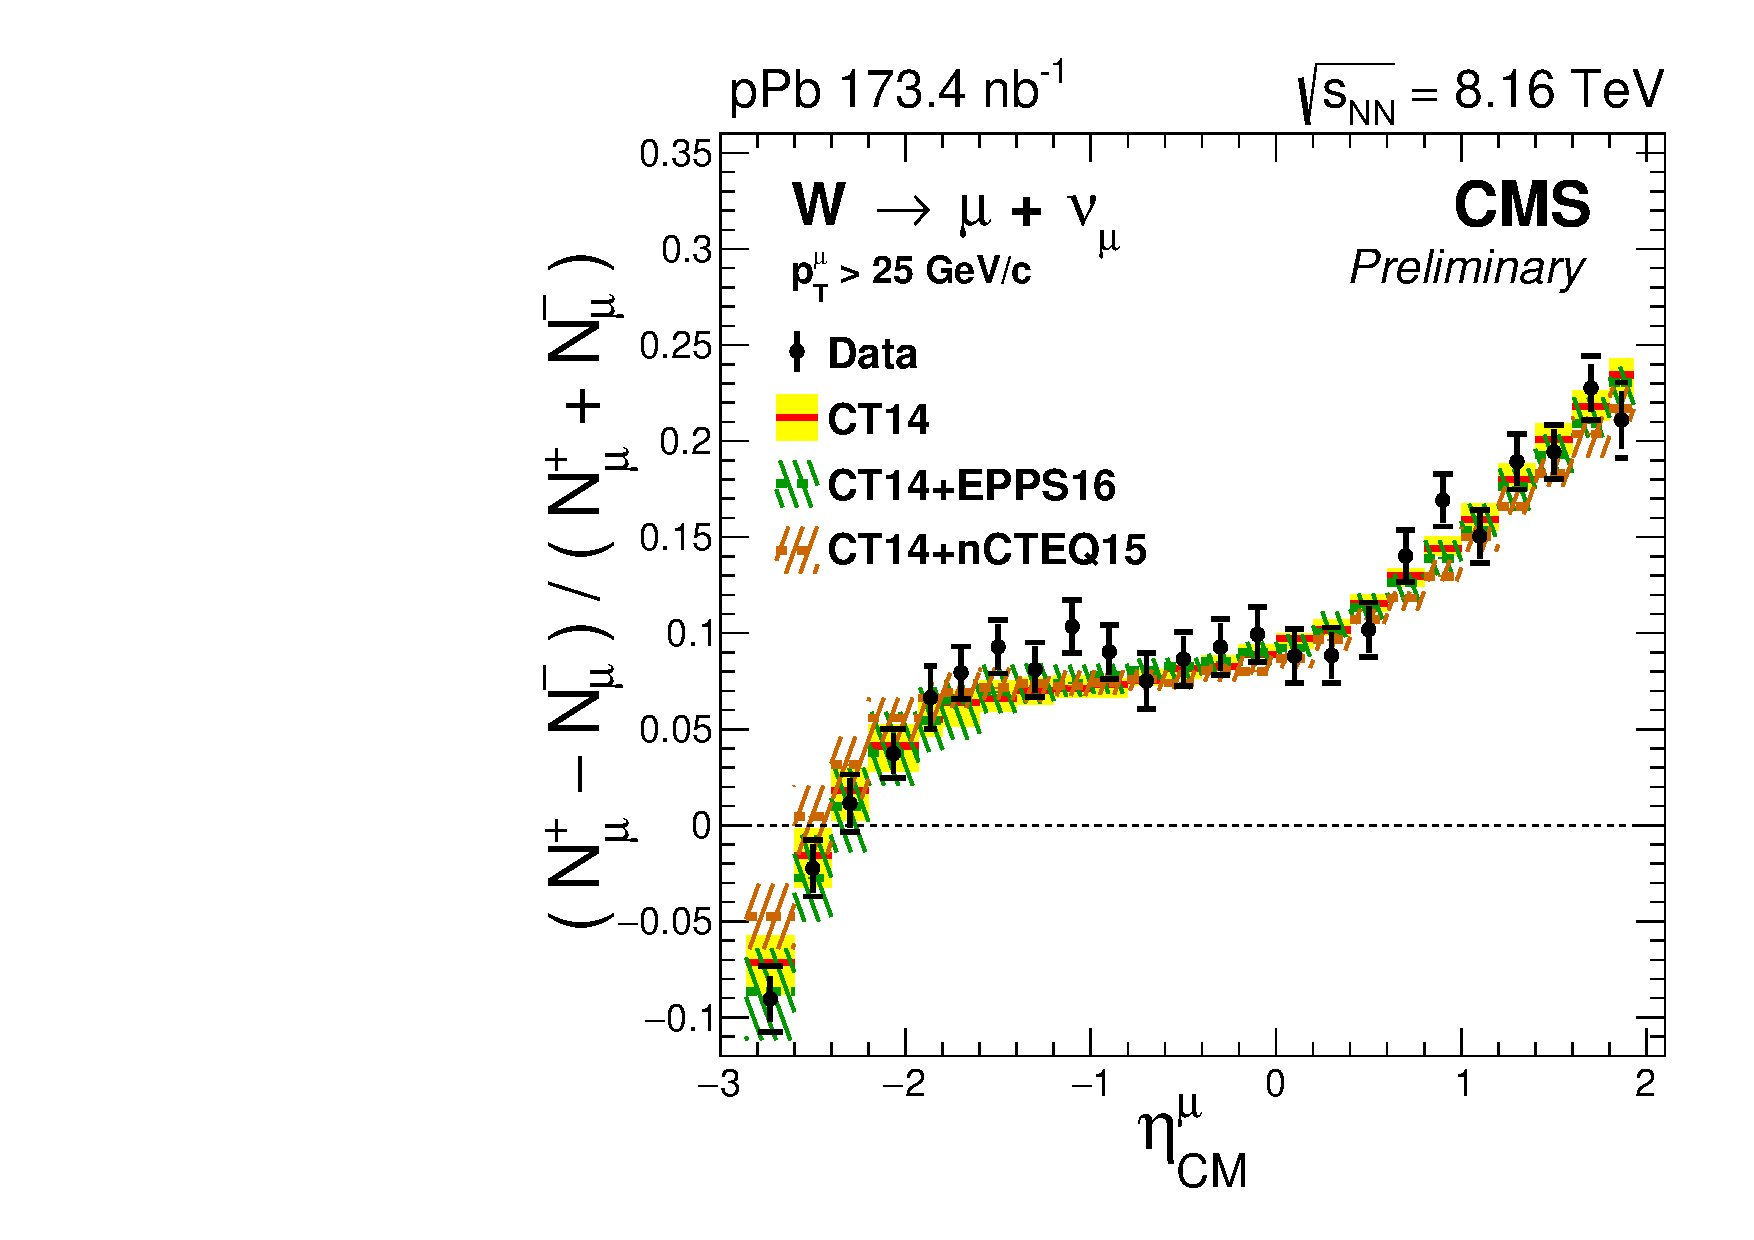
\includegraphics[width=0.55\textwidth]{Figures/WBoson/Results/Theory/gr_WToMuInc_PA_Charge_Asymmetry_EffTnP_NominalWithTheory_EPPS16.pdf}
 \caption{Muon charge asymmetry of $\WToMuNu$, given for each muon \etaMuCM range. Errors bars represent the statistical uncertainties, while the brackets represent the statistical and systematic uncertainties summed in quadrature. Theoretical predictions with (CT14+EPPS16 shown in dashed green line and CT14+nCTEQ15 shown in dashed brown line) and without (CT14, solid red line) PDF nuclear modifications are also shown, with the uncertainty bands. All theory uncertainty bands include the PDF uncertainties. }
 \label{fig:ChargeAsymmetry_WToMu_PA_Model}
\end{figure}

\begin{figure}[htb!]
 \centering
 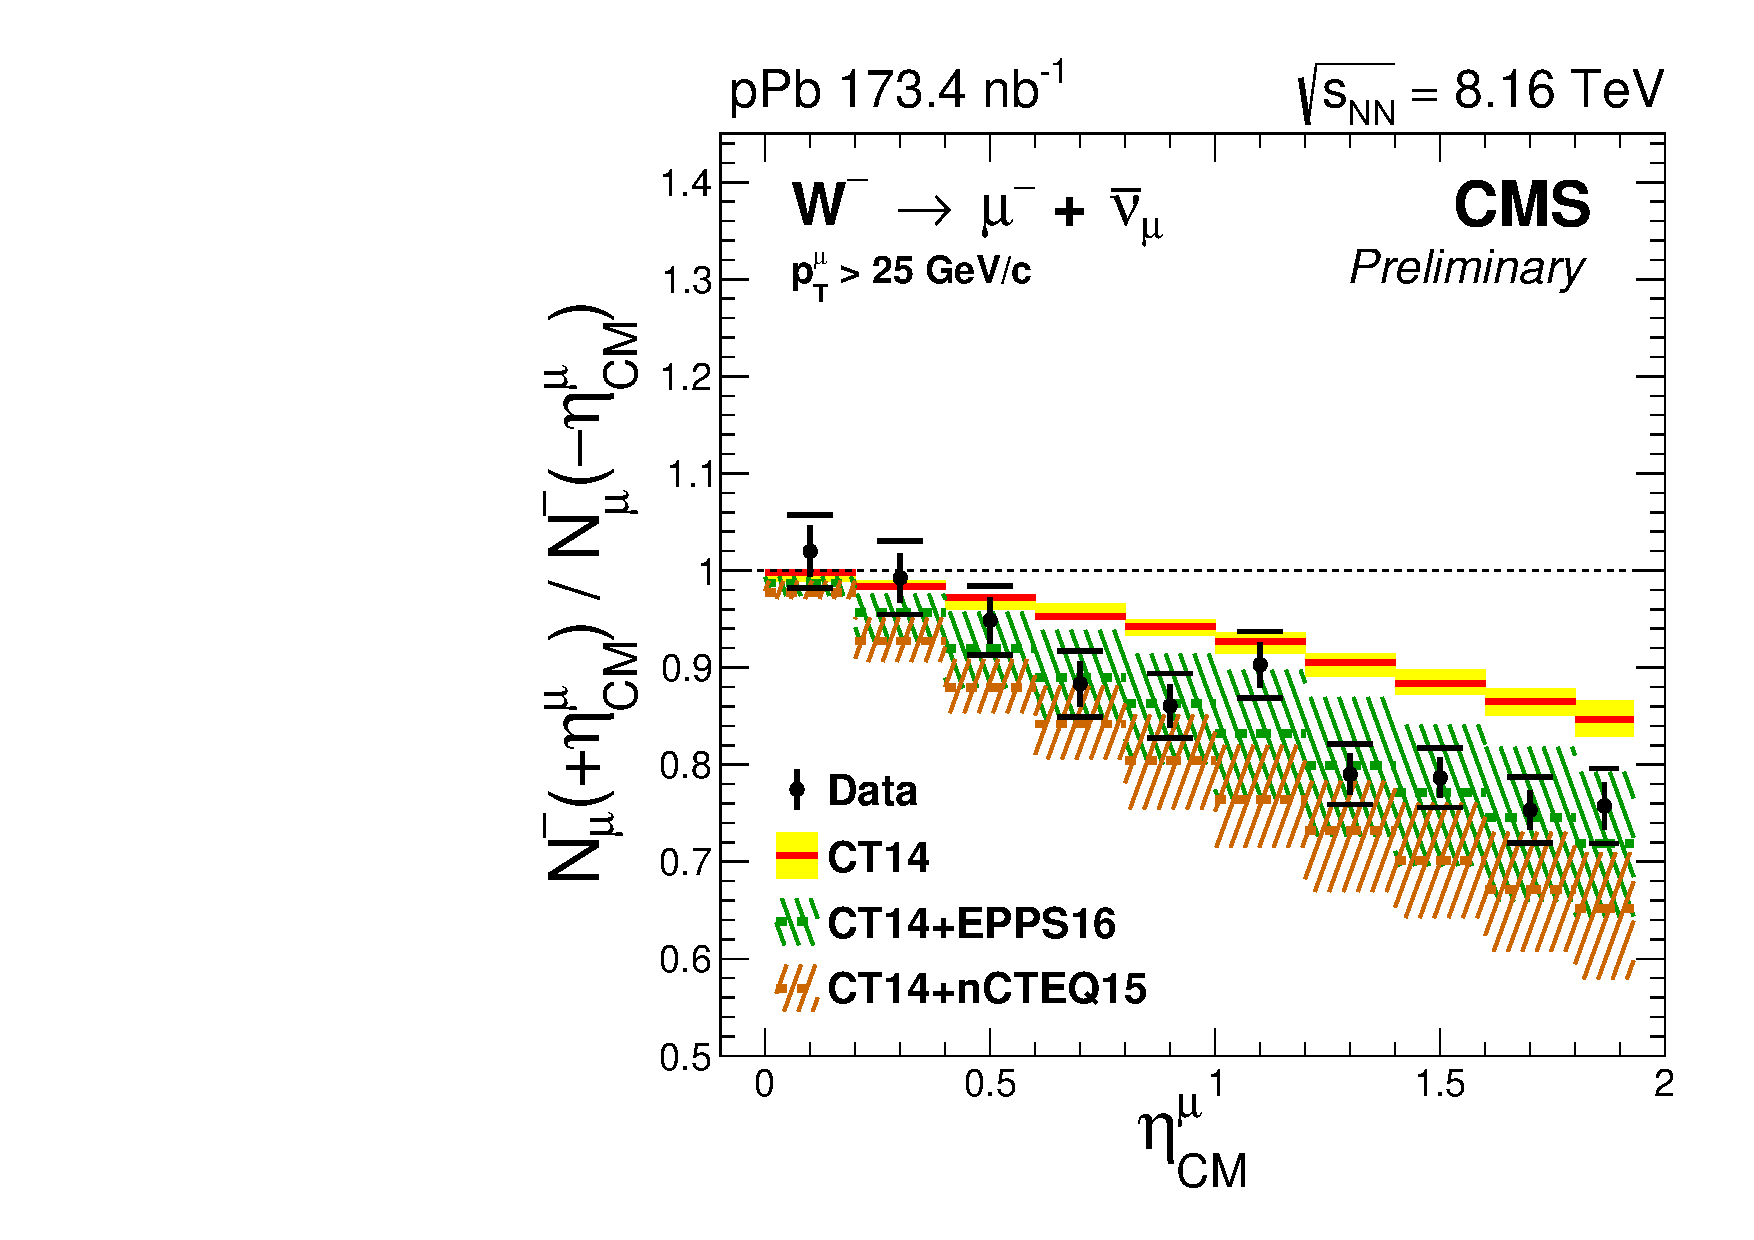
\includegraphics[width=0.45\textwidth]{Figures/WBoson/Results/Theory/gr_WToMuMi_PA_ForwardBackward_Ratio_EffTnP_NominalWithTheory_EPPS16.pdf}
%%
 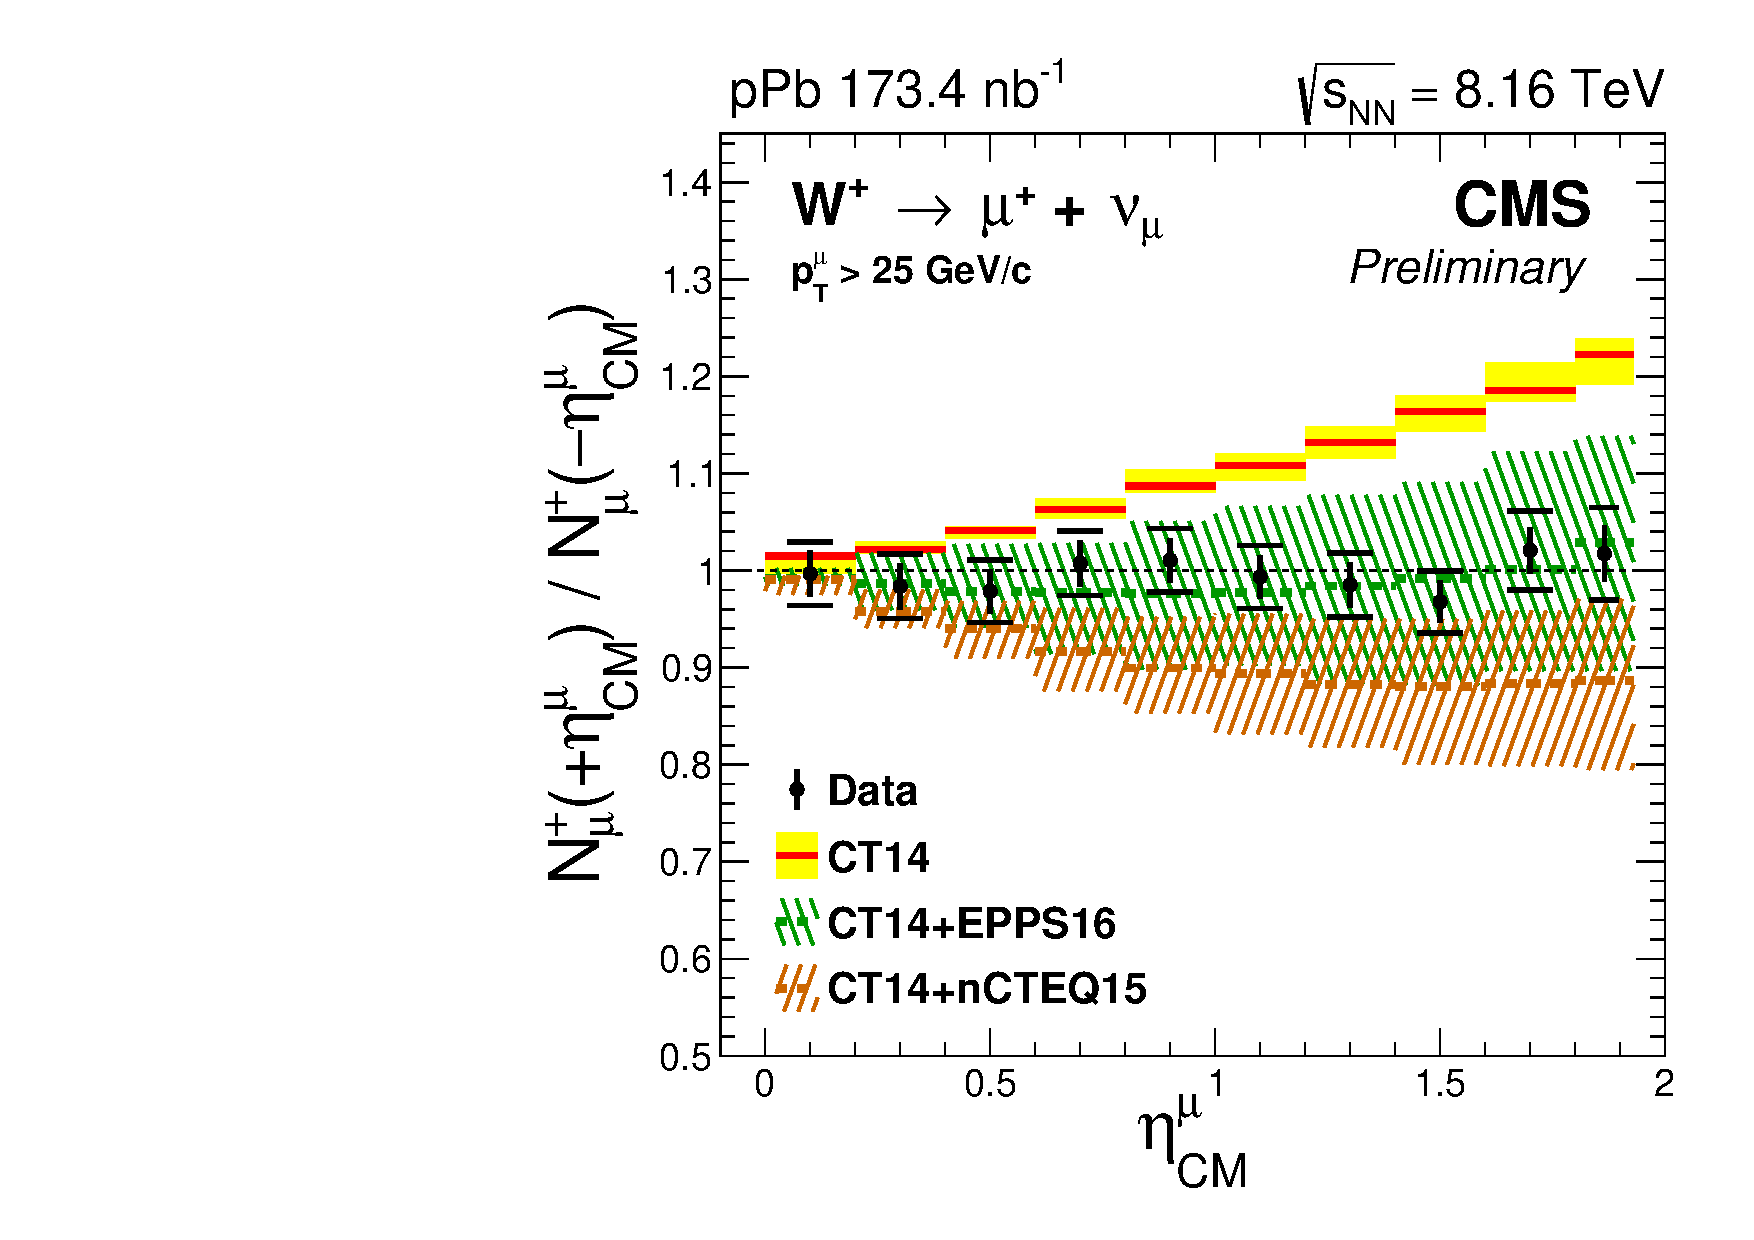
\includegraphics[width=0.45\textwidth]{Figures/WBoson/Results/Theory/gr_WToMuPl_PA_ForwardBackward_Ratio_EffTnP_NominalWithTheory_EPPS16.pdf}
%%
 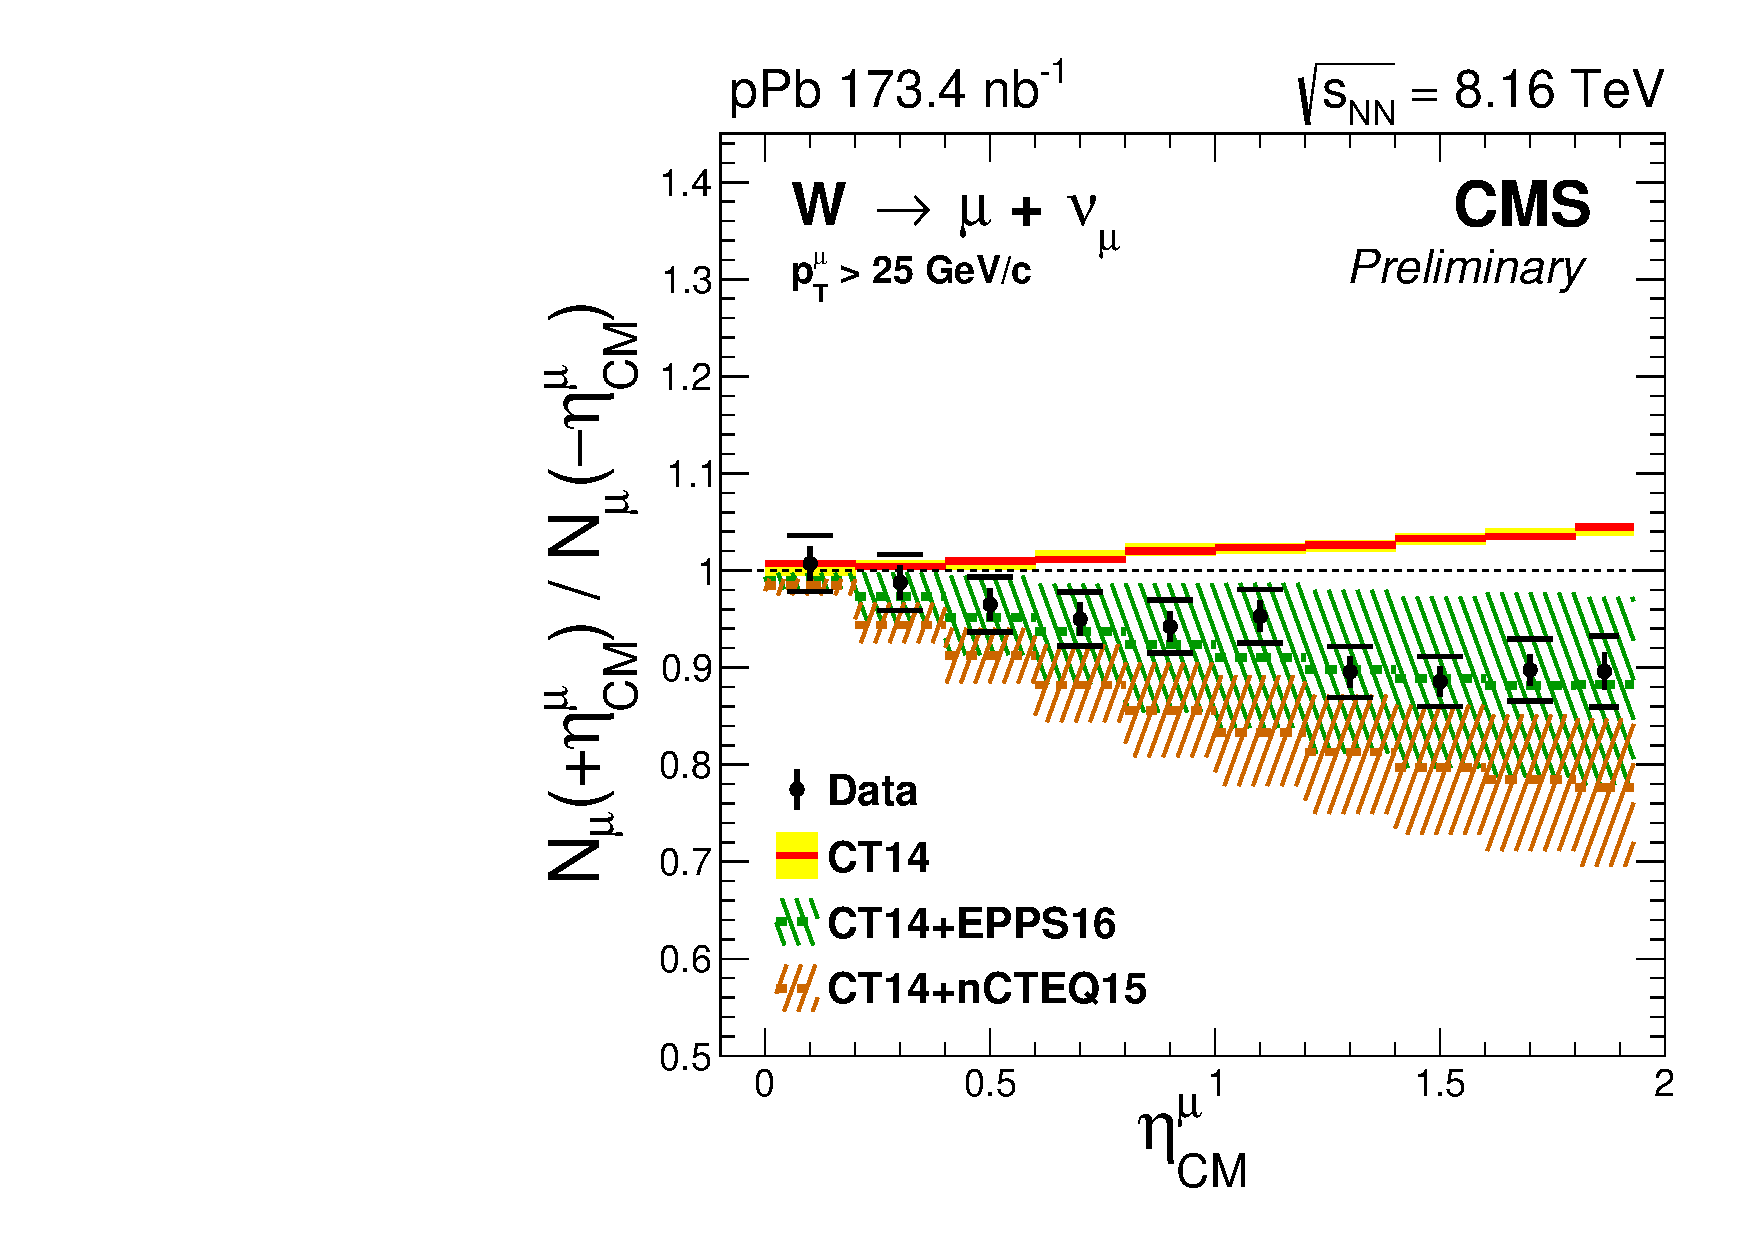
\includegraphics[width=0.45\textwidth]{Figures/WBoson/Results/Theory/gr_WToMuInc_PA_ForwardBackward_Ratio_EffTnP_NominalWithTheory_EPPS16.pdf}
 \caption{Forward-backward ratio of $\WToMuNu$, given for each muon \etaMuCM range separated in negative (top-left), positive (top-right) and all (bottom) charged muons. Errors bars represent the statistical uncertainties, while the brackets represent the statistical and systematic uncertainties summed in quadrature. Theoretical predictions with (CT14+EPPS16 shown in dashed green line and CT14+nCTEQ15 shown in dashed brown line) and without (CT14, solid red line) PDF nuclear modifications are also shown, with the uncertainty bands. All theory uncertainty bands include the PDF uncertainties. }
 \label{fig:ForwardBackwardRatio_WToMu_PA_Model}
\end{figure}

In order to quantify the level of agreement between each PDF calculation and the measurements of the \Wb-boson production in \RunpPb collisions, a $\chi^{2}$ test is performed according to:

\begin{equation}
 \chi^{2} = \sum_{i}\sum_{j}\left[\left(t(i) - d(i)\right)\cdot\left(\text{COV}_{\text{data}} + \text{COV}_{\text{theory}}\right)^{-1}\left[i , j\right]\cdot\left(t(j) - d(j)\right)\right]
 \label{eq:Chi2Test}
\end{equation}

where $t(i)$ is the value of the observable derived from the PDF calculation in bin $i$, $d(j)$ is the value of the observable measured in data in bin $j$, and $\left(\text{COV}_{\text{data}} + \text{COV}_{\text{theory}}\right)^{-1}$ is the inverse of the sum of the covariance matrices extracted from the data and PDF calculations. This approach takes into account the bin-to-bin correlations in both muon charge and pseudorapidity.

The outcome of the $\chi^{2}$ statistical test derived using the CT14 PDF, CT14+EPPS16 nPDF and CT14+nCTEQ15 nPDF calculations are summarized in \tab{tab:modelComparison_CT14}. The results of the CT14 PDF calculations are significantly disfavoured by the measurements, while the PDF calculations including nuclear modifications are in good agreement. In addition, the measurements tend to favour the nPDF calculations of the CT14+EPPS16 model over the ones from the CT14+nCTEQ15 model.

\begin{table}[htb!]
  \centering
  \resizebox{\textwidth}{!}{
  \renewcommand{\arraystretch}{1.5}
  \begin{tabular}{c *3c | *3c | *3c}
    \hline
    \multirow{2}{*}{Observable}  & \multicolumn{3}{c}{CT14} & \multicolumn{3}{c}{CT14+EPPS16} & \multicolumn{3}{c}{CT14+nCTEQ15} \\ \cline{2-10}
     & $\chi^{2}$ & ndf & Prob.($\%$) & $\chi^{2}$ & ndf & Prob.($\%$) & $\chi^{2}$ & ndf & Prob.($\%$) \\
    \hline
    $\dd\sigma(\WToMuNupm) / \dd\etaMuCM$ & 135 & 48 & $3\times10^{-8}$ & 32 & 48 & 96 & 40 & 48 & 79 \\
    $\left( N_{\mu}^{+} - N_{\mu}^{-} \right) \big/ \left( N_{\mu}^{+} + N_{\mu}^{-} \right)$ & 23 & 24 & 54 & 18 & 24 & 80 & 29 & 24 & 23  \\
    $N_{\mu}^{\pm}\left( +\etaMuCM \right) \big/ N_{\mu}^{\pm}\left( -\etaMuCM \right)$ & 98 & 20 & $3\times10^{-10}$ & 11 & 20 & 95 & 14 & 20 & 83  \\
    $N_{\mu}\left( +\etaMuCM \right) \big/ N_{\mu}\left( -\etaMuCM \right)$ & 87 & 10 & $2\times10^{-12}$ & 3 & 10 & 99 & 5 & 10 & 90  \\
    \hline
  \end{tabular}
  }
  \caption{Results of the $\chi^{2}$ statistical test between the measurements and the theory calculations from the CT14 PDF, CT14+EPPS16 nPDF and CT14+nCTEQ15 nPDF models. The value of the $\chi^{2}$, the number of degrees of freedom (ndf) and the $\chi^{2}$ probability (Prob.), are presented for the \WToMuNupm differential cross sections, the muon charge asymmetry, the \WToMuNupm forward-backward ratios, and the charge-summed forward-backward ratio, respectively.}
  \label{tab:modelComparison_CT14}
\end{table}




Considering the smaller size of the uncertainties of the measurements compared to those from the PDF models, the measurements have the potential to constrain the parametrisations of the EPPS16 nuclear modifications and the nCTEQ15 nuclear PDFs.


% END OF SUBSECTION